\documentclass{article}
\usepackage{graphicx} % Required for inserting images
\usepackage{graphicx} % Required for inserting images
%\usepackage[left=0.5in, right=0.5in, top=0.5in, bottom=0.5in]{geometry}
%\usepackage[left=1.5cm, right=1cm, top=0.5cm, bottom=1.5cm]{geometry}
\usepackage[left=1.5cm, right=1.5cm, top=0.5cm, bottom=1.5cm]{geometry}
\usepackage{amsmath}
\usepackage{amssymb}
\usepackage{amsfonts}
\usepackage{amsthm}
\usepackage{ulem}
\usepackage{bm}
\usepackage{tikz}
\usepackage{enumitem}

\date{}

\begin{document}
\fontsize{13}{15} \selectfont %This is 13pt text with 15pt line spacing.

\begin{center}
 \text{Potterhouse School. \hspace{1cm} Year 6 Math - Midterm Quiz III.} \qquad \\ 
\end{center} \\ 

Name: ...........................................................  \hspace{0.5cm}  Date: ....................... \hspace{0.5cm}  Class: ......\hspace{0.5cm} [40 marks]

\par
\vspace*{5pt} 
\textit{(You must show your working including the times tables of the divisors and multipliers.)  }
%\vspace{5pt}

\begin{center}
    \includegraphics[width=15cm]{Year_6_Mixed_Tests/Xx.png}
\end{center}
 \\

 \begin{enumerate}
 
\item \quad \( 4789 \div 5 \)   \hspace{2cm} [2 marks] 
\vspace{90pt}
\hline
\vspace{5pt}

\item \quad \( 5732 \times 6 \) \hspace{2cm} [2 marks]
\vspace{90pt}
\hline
\vspace{5pt}

\item \quad \text{What is the value of the 5 in this number? }  \( 54398\)  \hspace{2cm} [2 marks]
\vspace{40pt}

\begin{center}
\begin{tabular}{c@{\hspace{3cm}}c@{\hspace{3cm}}c@{\hspace{3cm}}c}
  5 & 50 & 50000 & 500 \\  
  \includegraphics[width=1cm]{cross.png} & 
  \includegraphics[width=1cm]{cross.png} & 
  \includegraphics[width=1cm]{cross.png} & 
  \includegraphics[width=1cm]{cross.png} \\
\end{tabular}
\end{center}
\hline
\vspace{10pt}

\item \quad \text{ What is 32691 rounded to the nearest Thousand? } \hspace{2cm} [2 marks]
\vspace{20pt}

\begin{center}
\begin{tabular}{c@{\hspace{3cm}}c@{\hspace{3cm}}c@{\hspace{3cm}}c}
  32000 & 33000 & 30000 & 40000 \\
  \includegraphics[width=1cm]{cross.png} & 
  \includegraphics[width=1cm]{cross.png} & 
  \includegraphics[width=1cm]{cross.png} & 
  \includegraphics[width=1cm]{cross.png} \\
\end{tabular}
\end{center}
\hline
\vspace{10pt}

\item \text{ Write these numbers in order of size. Start with the smallest. } \hspace{2cm} [2 marks] \\
\begin{center}
3.506\hspace{2cm}3.56\hspace{2cm}35.06\hspace{2cm}350.6\hspace{2cm}3.56 
\vspace{30pt}

.......\hspace{2cm}.....\hspace{2cm}.....\hspace{2cm}.....\hspace{2cm}.....  \\
\end{center}
\hspace {2cm} Smallest

\vspace{10pt}

\item \quad \text{ Fill in A, B, C and D in the number line below. } \hspace{2cm} [2 marks]
\vspace{10pt}

 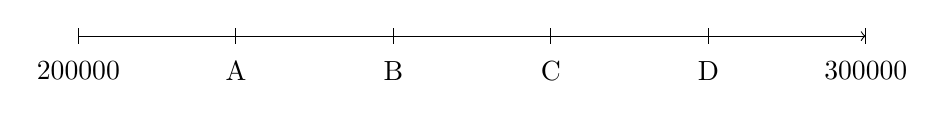
\begin{tikzpicture}
    % Draw the main line
    \draw[->] (0,0) -- (10,0);
    
    % Draw tick marks and labels
    \foreach \x/\label in {0/200000, 2/220000, 4/240000, 6/260000, 8/280000, 10/300000} {
        \draw (\x,-0.1) -- (\x,0.1);
        % Omit labels at positions 4 and 8 to leave them blank
        \ifnum\x=2 \else \ifnum\x=4 \else \ifnum\x=6 \else \ifnum\x=8 \else
            \node[below] at (\x,-0.2) {\label};
        \fi\fi\fi\fi
    }
    
    % Draw letters 'X' and 'Y' at positions 4 and 8
    \node[below] at (2,-0.2) {A};
    \node[below] at (4,-0.2) {B};
    \node[below] at (6,-0.2) {C};
    \node[below] at (8,-0.2) {D};
    
\end{tikzpicture}
\vspace{40pt}

\vspace{10pt}
\hline
\vspace{5pt}

% \item \quad \text{ Fill in A, B, C and D in the number line below. } 
% \vspace{40pt}

 % \begin{tikzpicture}
    % Draw the main line
   % \draw[->] (0,0) -- (10,0);
    
    % Draw tick marks and labels
   % \foreach \x/\label in {0/-400, 2/-200, 4/0, 6/200, 8/400, 10/600} {
       % \draw (\x,-0.1) -- (\x,0.1);
        % Omit labels at positions 4 and 8 to leave them blank
       % \ifnum\x=2 \else %\ifnum\x=4 \else 
      %  \ifnum\x=6 \else \ifnum\x=8 \else
     %       \node[below] at (\x,-0.2) {\label};
    %    \fi\fi\fi\fi
  %  }
    
    % Draw letters 'X' and 'Y' at positions 4 and 8
   % \node[below] at (2,-0.2) {A};
    %\node[below] at (4,-0.2) {B};
   % \node[below] at (6,-0.2) {C};
   % \node[below] at (8,-0.2) {D};
    
% \end{tikzpicture}

%\text{(9) Fill in X and Y in the number line below. } 
%\vspace{30pt}

 %\begin{tikzpicture}
    % Draw the main line
  %  \draw[->] (0,0) -- (10,0);
    
    % Draw tick marks and labels
   % \foreach \x/\label in {0/4000, 2/4200, 4/4400, 6/4600, 8/4800, 10/5000} {
    %    \draw (\x,-0.1) -- (\x,0.1);
        % Omit labels at positions 4 and 8 to leave them blank
     %   \ifnum\x=4 \else \ifnum\x=8 \else
      %      \node[below] at (\x,-0.2) {\label};
       % \fi\fi
    %}
    
    % Draw letters 'X' and 'Y' at positions 4 and 8
%   \node[below] at (4,-0.2) {A};
   % \node[below] at (8,-0.2) {B};
    
%\end{tikzpicture}

%\newpage

\item \quad \text{Write} \bm{\mathit{1147365}} \text{in words. } \hspace{2cm} [2 marks]
 %\text{(7) Write} \text{\textit{$\bm{38127}$}} \text{in words. } 
 \par
 \vspace{20pt}

\noindent \dotuline{\hspace{17cm}} \\
\par
\noindent \dotuline{\hspace{17cm}} \\
\vspace{10pt}
\hline
\vspace{10pt}

\item \quad \text{Write} \textit{\textbf{three million, five hundred and sixty-seven thousand, eight hundred and }} \\
\textit{\textbf{two}} \text{in digits.} \hspace{2cm} [2 marks]

 
 \par
 \vspace{60pt}
 ..............................................

 \vspace{20pt}
 \hline
 \vspace{10pt}

\item \quad \( 2 + 16 \div (9 - 1 ) \) \hspace{2cm} [2 marks]
\vspace{80pt}
\hline
\vspace{10pt}

%\item \quad \( 15 \div (3 + 2) \) 
%\vspace{60pt}
%\hline
%\vspace{5pt}


\item \quad \text{The Ghan train in Australia travels 1678 miles in a trip. How long does it travel in } \\ 
\quad \text{ 27 such trips?} \hspace{2cm} [2 marks]
\vspace{100pt}
\hline
\vspace{5pt}

\item \quad  \text{Ethan collected 1465 tanzanite stones. He would like to share them equally among 24 students.} \\ 
\quad \quad \text{(a) How many tanzanite stones will each student get?} \hspace{2cm} [1 mark] \\ 
\quad \quad \text{(b) How many will remain?} \hspace{2cm} [1 mark]
\vspace{120pt}
%\hline
\vspace{5pt}


\item \text{ Write these numbers in order of size. Start with the smallest. } \hspace{2cm} [2 marks] \\
\begin{center}
0.405 \hspace{3cm} 0.045 \hspace{3cm} \( \displaystyle \frac{4}{5} \) \hspace{3cm}45\%
\vspace{70pt}

 ..... \hspace{3cm} ..... \hspace{3cm}  ..... \hspace{3cm} .....     \\

\end{center}
\hspace{2 cm} smallest
\vspace{10pt}
\hline
\vspace{5pt}

\item \quad Add. \hspace{2cm} [2 marks]
\[
\begin{array}{cccccc}
& 4 & 2 & 6 & 1 & 8 \\
  & & 2 & 7 & 1 & 9 \\
+ & & & 3 & 8 & 2 \\
\hline
&  &  &  &  &  \\
\\ 
\hline 
\end{array}
\]

\vspace{10pt}
\hline
\vspace{5pt}

\item \quad Lay out and solve: \hspace{2cm} 27311 - 3798 \hspace{2cm} [2 marks]
\vspace{80pt}

\hline
\vspace{10pt}

\item \quad Lay out and solve: \hspace{2cm} 2.46 + 39.47 + 53.28 \hspace{2cm} [2 marks]
\vspace{80pt}

\hline
\vspace{10pt}
\vspace{5pt}

\item \quad Caleb caught bus D from the shop to the school. 
\begin{center}
    \includegraphics[width=10cm]{Year_6_Mixed_Tests/Bus_Timetable.png}
\end{center}
\\
(a) What time did she get to the school? \hspace{2cm} [1 mark] \\
\begin{center}
\begin{tabular}{c@{\hspace{3cm}}c@{\hspace{3cm}}c@{\hspace{3cm}}c}
  08:15 & 08:55 & 08:56 & 08:57 \\
  \includegraphics[width=1cm]{cross.png} & 
  \includegraphics[width=1cm]{cross.png} & 
  \includegraphics[width=1cm]{cross.png} & 
  \includegraphics[width=1cm]{cross.png} \\
\end{tabular}
\end{center}
%\hline
\vspace{10pt}

\newpage
\begin{flushleft}
 (b) How long did he take? \hspace{2cm} [1 mark] \\
 %(b) Which bus moved at the highest speed? \hspace{2cm} [1 mark] \\
 \vspace{50pt}
 (c) If he wanted to take 16 minutes in his journey, which bus would he take? \hspace{2cm} [1 mark] \\  
 %(c) Which bus took the longest time? \hspace{2cm} [1 mark] \\
 \vspace{50pt}
 (d) If he wanted to take 26 minutes in his journey , which bus would he take? \hspace{2cm} [1 mark] \\
 %(d) Which bus spent 16 minutes on the road? \hspace{2cm} [1 mark] \\
 \vspace{50pt}
 \end{flushleft}

\vspace{10pt}
\hline
\vspace{5pt}

\item \quad Here are the marks that Chemutai scored in her Scrabble game. \\
\begin{center}
16 \hspace{1cm} 28 \hspace{1cm}  26 \hspace{1cm}  27 \hspace{1cm}  30 \hspace{1cm}  31 \hspace{1cm}  26 \hspace{1cm}     
\end{center}

\begin{flushleft}
(a) What is the mode in the dataset? \hspace{2cm} [1 mark] \\
\vspace{50pt}

(b) What is the range of the dataset? \hspace{2cm} [1 mark] \\
\vspace{50pt}
(c) What is the mean of the dataset? \hspace{2cm} [1 mark] \\
\vspace{50pt}
(d) What is the median of the dataset? \hspace{2cm} [1 mark] \\
\vspace{50pt}
\end{flushleft}

\hline
\vspace{5pt}

%\item Vicky’s class kept a record of how many students had a packed lunch each day for 
%a week. They displayed the information in this dual bar chart. \\
%\begin{center}
 %   \includegraphics[width=10cm]{Year_6_Mixed_Tests/Bar_Graph_Boys_Girls.png}
%\end{center}
\\
%How many packed lunches in total did the girls have this week?

%\begin{center}
%\begin{tabular}{c@{\hspace{3cm}}c@{\hspace{3cm}}c@{\hspace{3cm}}c}
 % 130 & 240 & 250 & 490 \\
 % \includegraphics[width=1cm]{cross.png} & 
 % \includegraphics[width=1cm]{cross.png} & 
 % \includegraphics[width=1cm]{cross.png} & 
 % \includegraphics[width=1cm]{cross.png} \\
%\end{tabular}
%\end{center}

\item \quad This clock shows the time a game will start in the evening.
\begin{center}
    \includegraphics[width=4.5cm]{Year_6_Mixed_Tests/Clock2.png}
\end{center}
\begin{flushleft}
(a) What wass the time 30 minutes earlier in 12 hour time? \hspace{2cm} [1 mark] \\
\vspace{20pt}
%(b) How would this time be shown in 24 hour time? \hspace{2cm} [1 mark] \\
%\vspace{50pt}
(b) What will be the time after 14 minutes in 24 hour time? \hspace{2cm} [1 mark]
\vspace{20pt}
%(c) What will be the time after 12 minutes? \hspace{2cm} [1 mark]
\end{flushleft}

 
%\begin{table}
 %   \centering
  %  \begin{tabular}{|c|c|c|c|c|}
   % \hline
    %    1 & 3 & 5 & 7 & \hline \\
     %    4& 6 & 7 & 8 & \hline 
      %   \hline
    % \end{tabular}
    % \caption{Caption}
    % \label{tab:new}
% \end{table}

\end{enumerate}

\end{document}
